\chapter{VBTE}
Følgende afsnit beskriver VBTE'ens hardware i de enkelte blokke, grænsefladerne derimellem samt funktionen af blokkene. Derudover er der implementeret et testdisplay samt mulighed for manuelt at indstille I2C adressen. Disse er kun ment til test og er derfor ikke dokumenteret.
\section{Overordnet design}
Nedenfor ses det overordnede hardware blokdiagram. Herefter følger en beskrivelse af de forskellige blokke samt signaler.
\begin{figure}[H]
\centering
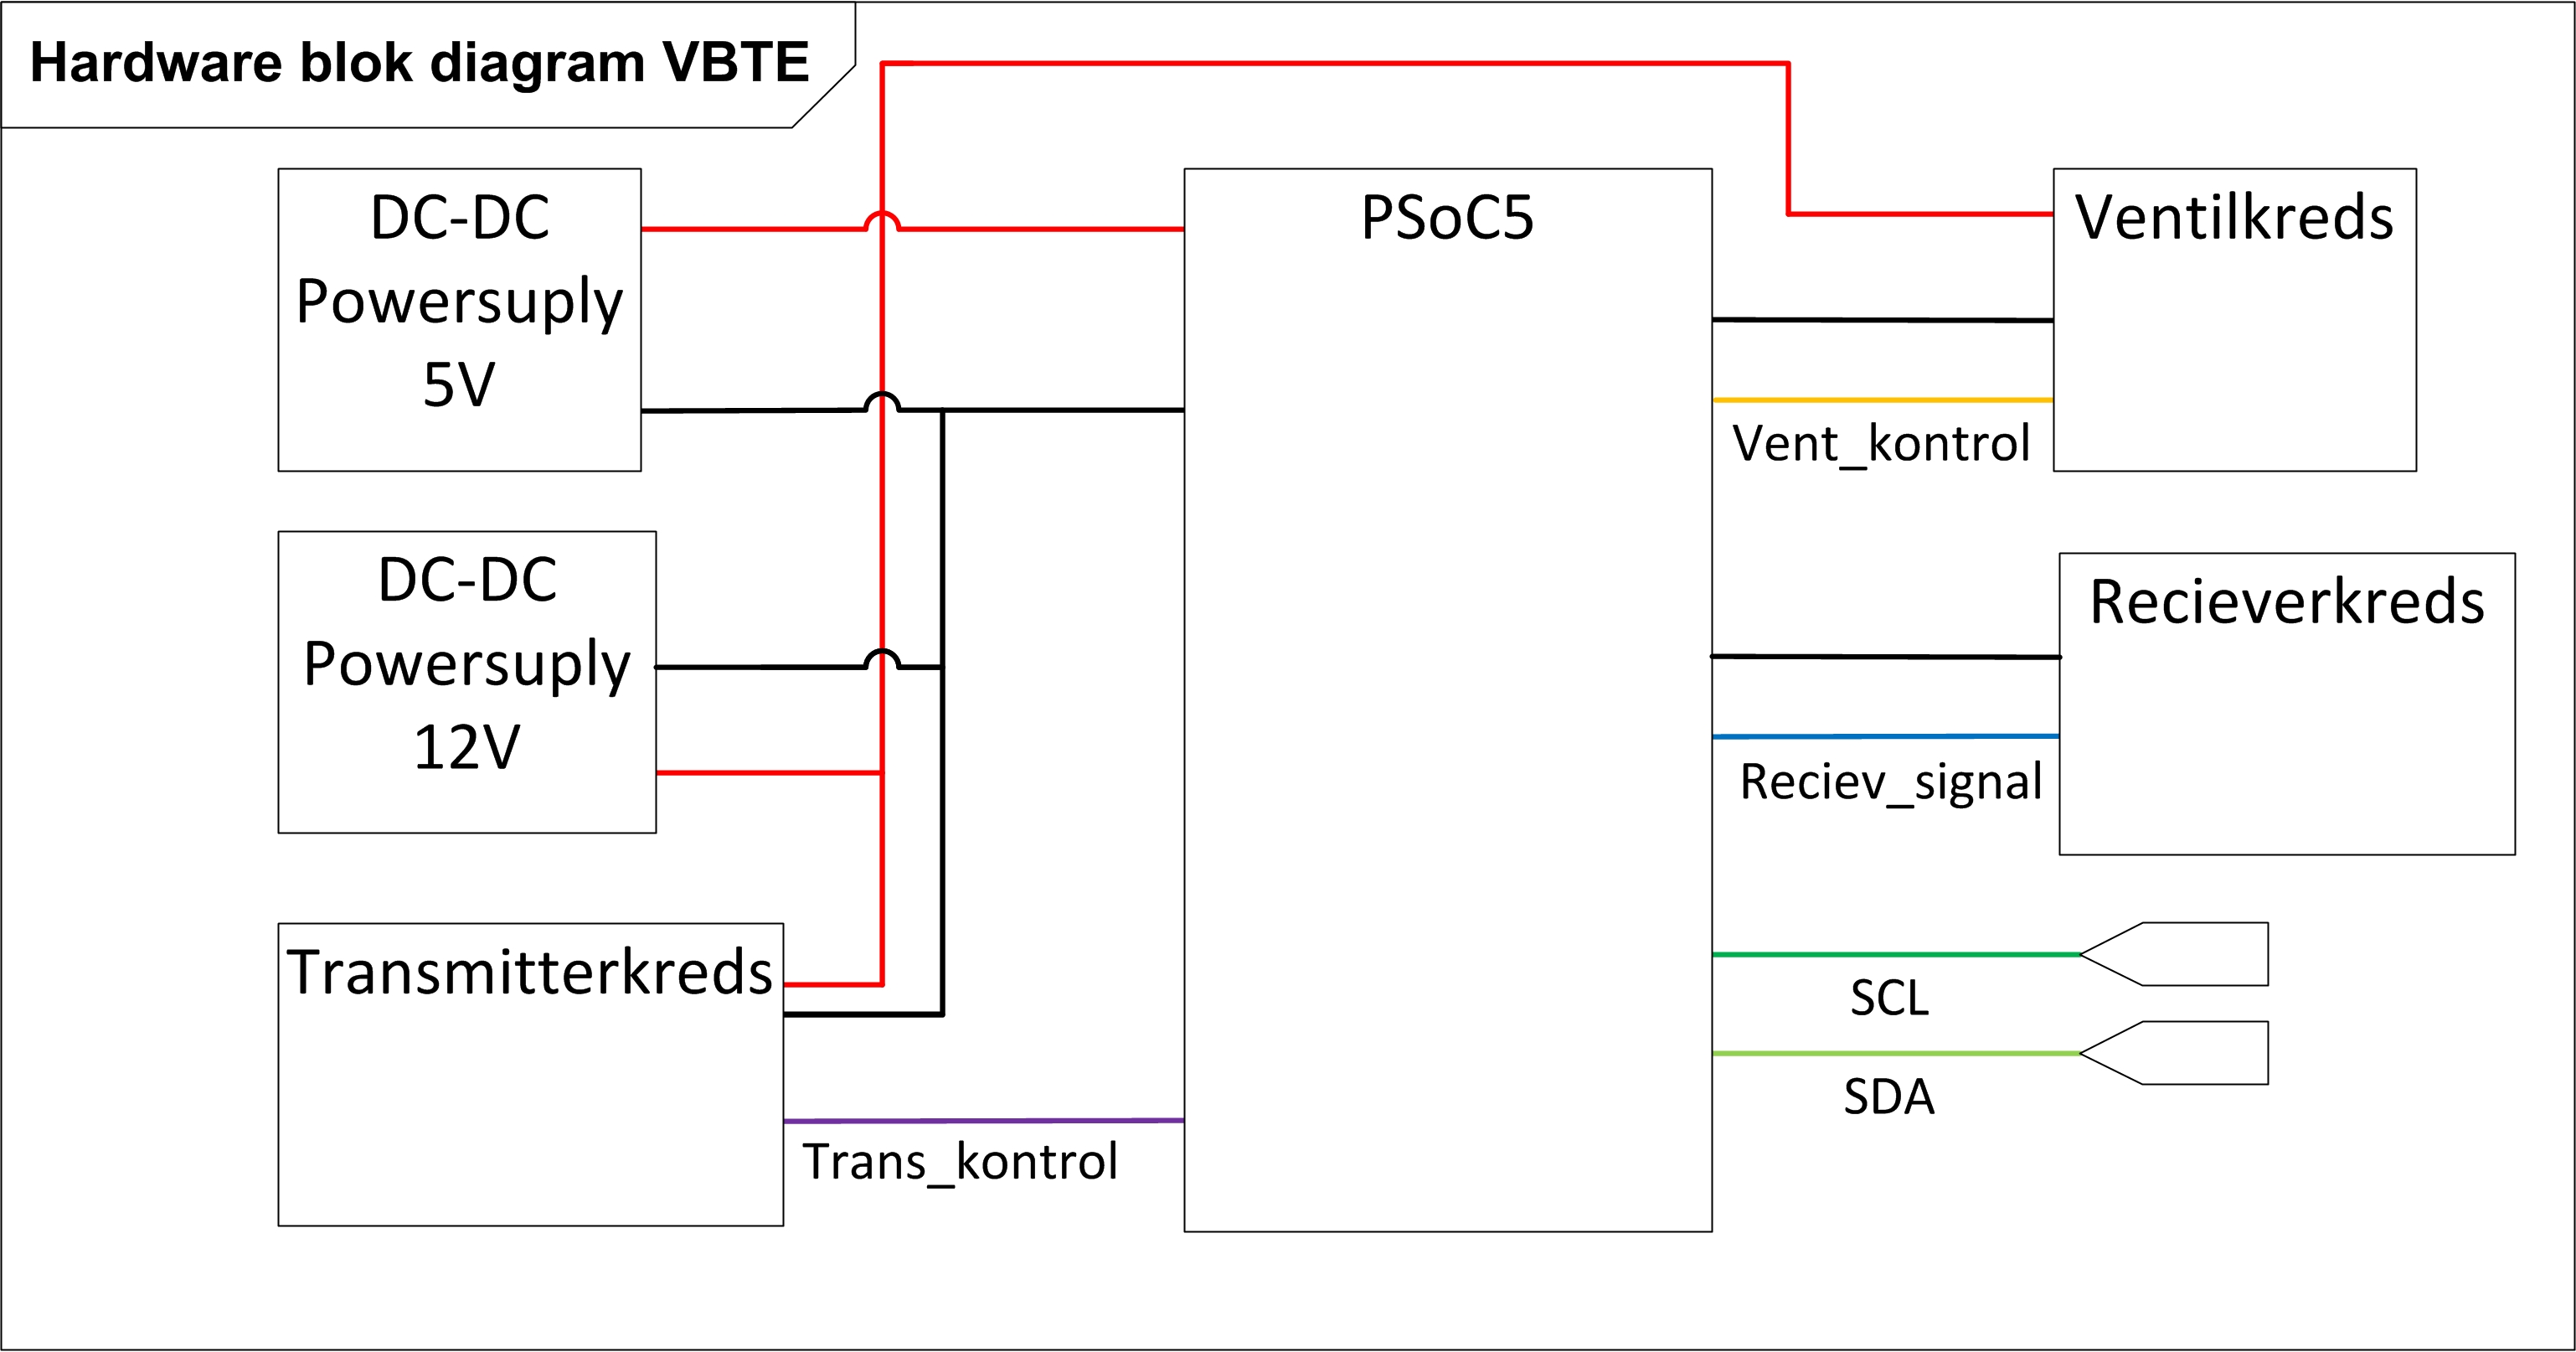
\includegraphics[width=1\textwidth]{billeder/HWVBTE}
\caption{Overordnet blokdiagram for VBTE hardware}
\label{fig:HWVBTE}
\end{figure}
\subsection{Blokke}
Nedenfor beskrives de enkelte blokke illustreret på \textit{Figur~\ref{fig:HWVBTE}}
\subsubsection{PSoC5}
PSoC'en er den centrale del af VBTE'en og står for styringen af hele VBTE'en. Den består af:
\begin{itemize}
\item MicroController
\item PGA
\item Mixer
\item Timer
\item Clocks
\item I2C
\item Delta-Sigma ADC
\item Kontrolregister
\end{itemize}
PSoC'en er et færdigkøbt produkt og for detaljer om de enkelte blokke heri henvises der til databladet for PSoC5.
\subsubsection{DC-DC powersuply 5V}
Se powersuply afsnittet.
\subsubsection{DC-DC powersuply 12V}
Se powersuply afsnittet.
\subsubsection{Transmitterkreds}
Transmitterkredsen består af en MOSFET samt en keramisk ultralyds transmitter(Model: 400ST). Kredsen bliver drevet af 12V powersuply. \fxnote{Skal ligge i opbygningen af blokken i stedet for her}
\subsubsection{Reciverkreds}
Recierkredsen består af en keramisk ultralyds reciver(Model: 400SR).
\subsubsection{Ventilkreds}
Ventilkredsen består af en MOSFET samt en ventil(Model: EV210A-1.2 og EV210A-4.5)
\newpage
\section{Nedbrydning af blokke}
Nedenfor følger nedbrydningen af de enkelte blokke med henblik på at designe de enkelte dele til systemet. Nedbrydningen sker for at gøre designet nemmere og mere overskueligt.
\subsection{PSoC5}
På \textit{Figur \ref{fig:PSoCBlok}} ses HW-designet internt på PSoC'en. De enkelte blokke bliver beskrevet efterfølgende.
\begin{figure}[H]
\centering
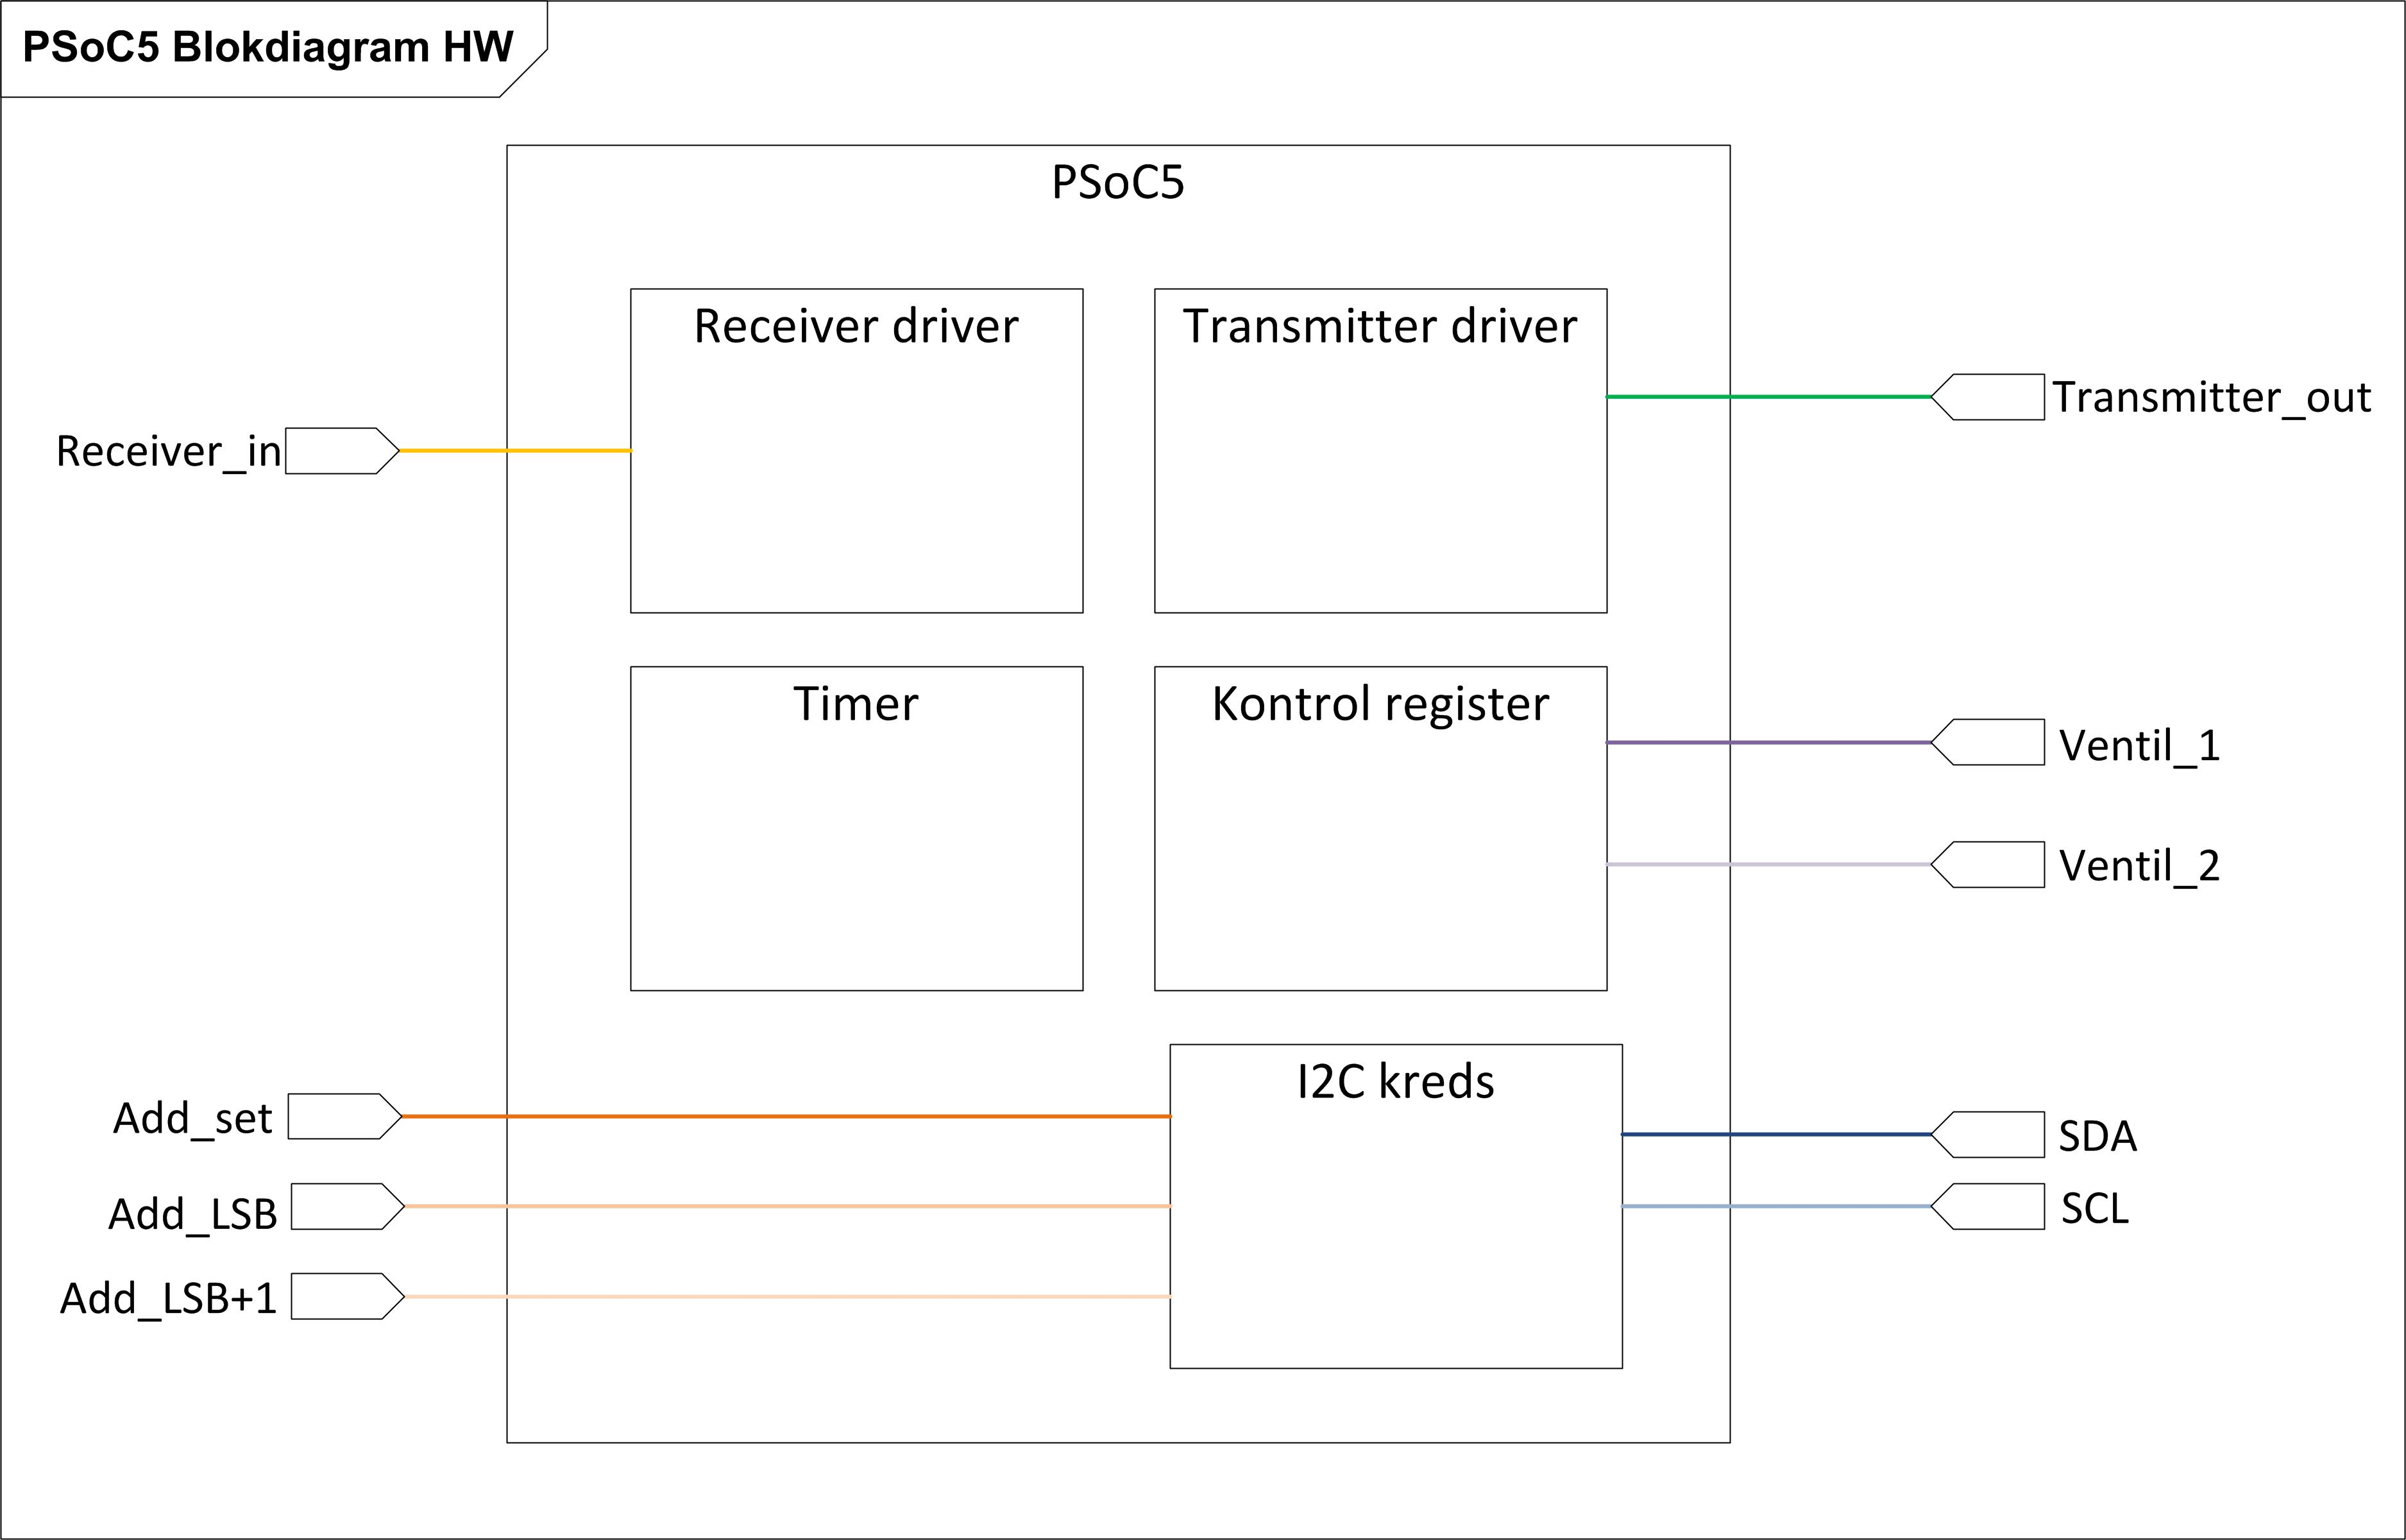
\includegraphics[width=1\textwidth]{billeder/PSoCBlock}
\caption{PSoC5 blokdiagram}
\label{fig:PSoCBlok}
\end{figure}
\subsubsection{Signalbeskrivelser:}
For signalbeskrivelser se \textit{tabel \ref{table:PSoCSignaler}}.
\fxnote{OPDATER TABELLEN!!!!}
\begin{table}[H]
\begin{tabular}{|p{3cm}|p{3cm}|p{3cm}|p{4.5cm}|} \hline
\cellcolor[gray]{0.85}Signal navn& \cellcolor[gray]{0.85}Type &\cellcolor[gray]{0.85}Spænding&\cellcolor[gray]{0.85}Beskrivelse\\ \hline
Receiver\_in & Analog (AC = 40kHz) & Ligger fra ca 0.01V til 0.3V & Spænding genereret i ultralydsreceiveren.\\ \hline
Transmitter\_out & Analogt (AC = 40kHz) & ~0V til ~5V & Signal der skal styre ultralydstransmitteren \\ \hline
Vent\_1 & Digitalt & ~0V til ~5V & Signal der skal styre ventilen til at lukke vand ind med.\\ \hline
Vent\_2 & Digitalt & ~0V til ~5V & Signal der skal styre ventilen til at lukke vand ud med.\\ \hline
SDA & Digitalt & ~0V til ~5V & Et digitalt signal mellem VBTE og SM hvor I2C data læses fra.\\ \hline
SCL & Digitalt & ~0V til ~5V & Digitalt clocksignal til I2C.\\ \hline
Add\_set & Digitalt & ~0V til ~5V & Digitalt signal til at sætte I2C adressen. \\ \hline
Add\_LSB & Digitalt & ~0V til ~5V & Digitalt signal til at sætte LSB i I2C adressen. \\ \hline
Add\_LSB+1 & Digitalt & ~0V til ~5V & Digitalt signal til at sætte LSB i I2C adressen.\\ \hline
\end{tabular}
\caption{Tabel over signaler i PSoC blokken}
\label{table:PSoCSignaler}
\end{table}
\subsubsection{Blokbeskrivelser:}
\subsubsection{Timer}
Timeren skal holde øje med tiden. Dette skal ske ved at timeren skal køre hele tiden. Der bliver læst timerværdien når et burst bliver sendt og når et burst bliver modtaget. Timeren skal derfor have en forholdsvis hurtig clock for at kunne gøre afstandsmålingen hurtig nok.
\subsubsection{I2C kreds}
I2C kredsen skal stå for I2C interfacet mellem SM og KI. I2C protokollen kører 5V og med pull-up modstande. Denne del håndteres dog på SM. I2C'en benytter standard I2C protokol, og for yderligere info om data henvises der til \textit{Systemarkitektur/protokoller/I2C}.
\subsubsection{Receiver Driver}
Receiver driveren modtager signalet fra ultralydsrecieveren. Signalet skal, når det modtages, løftes op til 2.5V for at det kan anvendes på PSoC'en samt forstærkes. Det er vigtigt at signalet bliver tydeligt nok til at man kan være sikker på at man har modtaget en detektion. 
\subsubsection{Transmitter Driver}
Det er vigtigt ved transmitteren at frekvensen ligger ret præcist da den dæmper rigtigt meget ikke ret langt væk fra 40kHz. For at timingen skal virke skal der også laves så der kan stoppes når der er sendt 10 perioder.
\subsubsection{Ventil Driver}
Ventil driveren er den mest simple driver. Denne skal blot bære et digitalt signal til ON og OFF på hhv. ventilen til at lukke vand ind og ventilen til at lukke vand ud.

\subsection{Transmitter kreds}
På \textit{figuren \ref{fig:transmitterblok}} ses nedbrydningen af Transmitter kreds-blokken. Transmitterkredsen omsætter et kontrolsignal fra PSoC'en til et ultralyds signal.
\begin{figure}[H]
\centering
\includegraphics[scale=1]{billeder/transmitterblok}
\caption{På figuren ses transmitter blokken nedbrudt}
\label{fig:transmitterblok}
\end{figure}
\subsubsection{Signalbeskrivelser}
Signalerne internt i transmitter kredsen ses i \textit{tabel \ref{table:transmitterblok}}
\begin{table}[H]
\begin{tabular}{|p{3cm}|p{3cm}|p{3cm}|p{4.5cm}|} \hline
\cellcolor[gray]{0.85}Signal navn& \cellcolor[gray]{0.85}Type &\cellcolor[gray]{0.85}Spænding&\cellcolor[gray]{0.85}Beskrivelse\\ \hline
Trans\_kontrol & Digitalt & 0V - 5V & Modtages fra PSoC'en og skal omsættes til en større spænding over ultralydstransmitteren.\\ \hline
Trans\_out & Analogt (lyd) & 120dB & Dette signal er lyden fra ultralydstransmitteren der sendes mod vandet og reflekteres tilbage til receiveren. \\ \hline
12V forsyning & Analogt DC & 12V$\pm$0.1V & 12V forsyning der leveres for powersupplyen beskrevet under powersupply.\\ \hline
GND & Ground & 0V & Ground i systemet \\ \hline
\end{tabular}
\caption{Tabel over signaler i Transmitterblokken}
\label{table:transmitterblok}
\end{table}

\subsection{Ventil Kreds}
Ventil kredsen får to kontrolsignaler fra PSoC'en der skal åbne for hver sin ventil. Kredsen skal sørge for at ventilerne kan få lov til at trække den strøm der er nødvendig for at drive dem. På \textit{figur \ref{fig:ventilblok}} ses blokdiagrammet for ventilkredsen. Signalerne på blokdiagrammet er beskrevet i \textit{tabel \ref{table:ventrilkreds}}
\begin{figure}[H]
\centering
\includegraphics[scale=1]{billeder/ventilblok}
\caption{På figuren ses ventilblokken nedbrudt}
\label{fig:ventilblok}
\end{figure}
\begin{table}[H]
\begin{tabular}{|p{3cm}|p{3cm}|p{3cm}|p{4.5cm}|} \hline
\cellcolor[gray]{0.85}Signal navn& \cellcolor[gray]{0.85}Type &\cellcolor[gray]{0.85}Spænding&\cellcolor[gray]{0.85}Beskrivelse\\ \hline
Ventil\_1\_kontrol & Digitalt & 0V - 5V & Modtages fra PSoC'en og skal omsættes til en større spænding over ventilen.\\ \hline
Ventil\_2\_kontrol & Digitalt & 0V - 5V & Modtages fra PSoC'en og skal omsættes til en større spænding over ventilen.\\ \hline
Ventil\_1\_out & Digitalt & 0V - 12V & Udgangsspænding til ventilen.\\ \hline
Ventil\_2\_out & Digitalt & 0V - 12V & Udgangsspænding til ventilen.\\ \hline
12V forsyning & Analogt DC & 12V$\pm$0.1V & 12V forsyning der leveres for powersupplyen beskrevet under powersupply.\\ \hline
GND & Ground & 0V & Ground i systemet \\ \hline
\end{tabular}
\caption{Tabel over signaler i Transmitterblokken}
\label{table:ventrilkreds}
\end{table}
